\chapter{Architettura generale del sistema} \label{cap:architettura-generale}

\section{Topologia generale} \label{sec:topologia_generale}

Per la definizione di questo sistema software è stato scelto di utilizzare un'architettura a microservizi, in quanto permette di avere un sistema scalabile e flessibile. Il pattern topologico scelto è quello REST.

Sono presenti all'interno del sistema due parti principali. Una parte è dedicata all'interazione con l'utente, l'altra parte è dedicata alla gestione dei dati e della logica di business, tra cui la comunicazione con i sistemi esterni quali lampioni, sensori e api meteo.

Ognuna delle responsabilità del sistema è stata suddivisa in un microservizio come segue:

\begin{itemize}
    \item \textbf{WebApplication}: è il microservizio che si occupa di gestire l'interazione con l'utente;
    \item \textbf{Anagrafica}: è il microservizio che si occupa di gestire i dati anagrafici dei lampioni, dei gruppi e delle aree in cui questi sono collocati;
    \item \textbf{Coordinazione}: è il microservizio che si occupa di gestire l'accensione e lo spegnimento dei lampioni secondo regole specifiche e utilizzando le informazioni provenienti dai sensori e da api varie per ottimizzare l'illuminazione;
    \item \textbf{Autenticazione}: è il microservizio che si occupa di gestire l'autenticazione degli utenti e di fornire i token necessari per l'accesso agli altri servizi;
    \item \textbf{logging}: è il microservizio che si occupa di gestire i log dei lampioni e dei sensori. Da questi, inoltre, vengono estratte informazioni necessarie per la gestione dell'illuminazione e più in generale aggregazioni di dati utli per l'analisi e la presentazione all'utente.
\end{itemize}

Possiamo definire queste responsabilità come dei componenti. Ognuno di questi componenti ha un'interfaccia ben definita e può essere sostituito con un altro componente che implementa la stessa interfaccia. Questo ci permette di utilizzare al massimo le pratiche di CICD.

I componenti dell'applicazione, le interfacce utilizzate ed esposte e le funzionalità fornite sono mostrate in figura \ref{fig:high-level-diagram}.

\begin{figure}[ht]
    \centering
    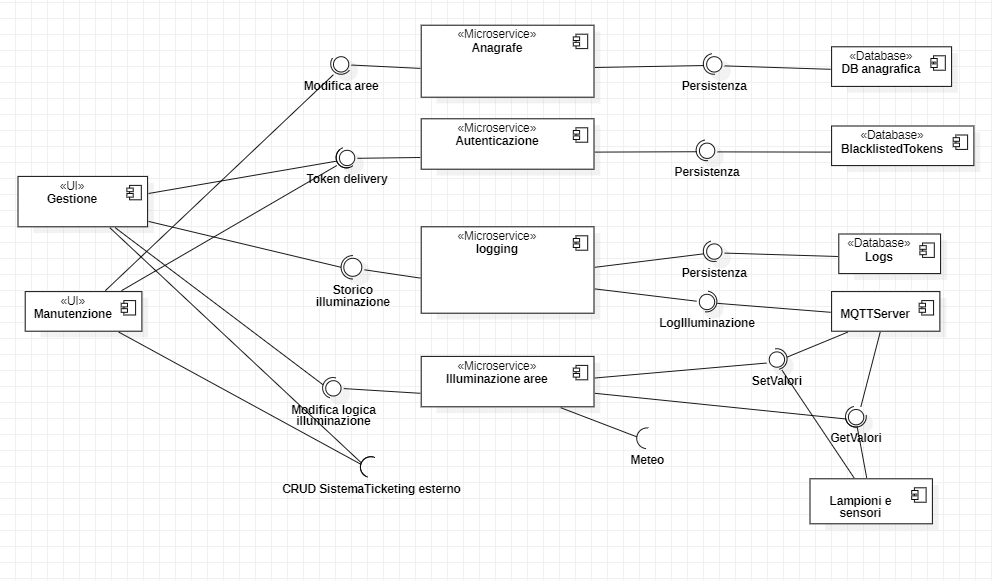
\includegraphics[width=\textwidth]{img/high-level-diagram.png}
    \caption{Diagramma dei componenti del sistema generale}
    \label{fig:high-level-diagram}
\end{figure}


\section{User interface}

Come user Interface è stato scelto di utilizzare un'interfaccia web. Questa è stata scelta in quanto permette di avere un'interfaccia accessibile da qualsiasi dispositivo e non richiede l'installazione di software aggiuntivo. Inoltre, permette di avere un'interfaccia che può essere facilmente aggiornata e modificata.

Per l'implementazione é stato scelto di utilizzare il framework Angular.

La scelta di utilizzare una webapp come interfaccia utente risponde inoltre ai requisiti di vincolo: \textbf{RV\_01}, \textbf{RV\_02}, \textbf{RV\_03}, \textbf{RV\_04}, \textbf{RV\_05}.

In poche parole l'applicazione deve essere utilizzabile da mobile e dai maggiori browser nelle versioni più recenti. Questa è la definizione data dai requisiti sopra citati.

\section{Business backend e microservizi}

Il business backend è il componente che si occupa di gestire la logica di business dell'applicazione. Questo componente è composto dai microservizi citati precedentemente alla sezione \ref{sec:topologia_generale}.

La scelta di suddividere per responsabilità i microservizi serve a rispondere al requisito di vincolo \textbf{RV\_06}, ovvero che il sistema deve essere scalabile orizzontalmente. Questi Microservizi sono infatti inoltre anche gestiti in modo tale da rimanere stateless rispetto all'utente ed utilizzando per ciascuno un database separato. In caso di aumenti di carico del sistema è quindi semplicemente necessario aggiungere nuove istanze dei microservizi.

Avendo poi basi di dati ridotte ed utilizzando però DBMS relazionali per via della loro facilità d'utilizzo non è necessario dover creare complesse strategie di sharding per la suddivisione del carico.

\subsection{DNS}

Per la struttura posta dietro alla REST based architecture, ci sarà bisogno di una definizione di nomi di dominio. Questa definizione è necessaria per poter utilizzare le risorse specifiche di ogni microservizio senza utilizzare un livello intermedio di API.

